\bigskip 
\bigskip 
\subsubsection{Contenido}
\bigskip 
%\begin{wrapfigure}{r}{0.5\textwidth}
%  \begin{center}
%    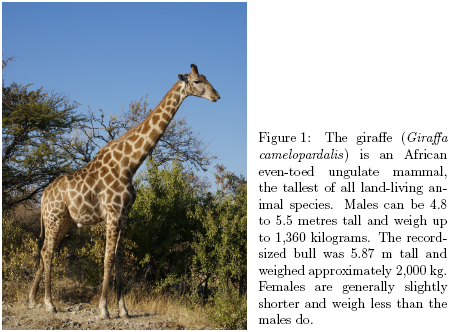
\includegraphics[width=0.48\textwidth]{./ingles/Latex_example_sidecap.jpg}
%  \end{center}
%\end{wrapfigure}

\begin{description}
\item[Nombre:] Born to be British
\item[Cristaleria:] Rock glass (6oz / 180cc)
\item[M\'etodo de elaboraci\'on:] Batido
\item[Decoraci\'on:] Rodajas de manzana
\end{description}

\begin{table}[h]
\caption{Ingredientes y proporciones} 
\label{tab:fonts}
\begin{center}       
\begin{tabular}{|l|l|l|c|l|} %% this creates two columns
%% |l|l| to left justify each column entry
%% |c|c| to center each column entry
%% use of \rule[]{}{} below opens up each row
\hline
\rule[-1ex]{0pt}{3.5ex}  \textbf{Producto} & \textbf{Bebida} & \textbf{Marca} & \textbf{Volumen} & \textbf{Fraccion}  \\
\hline
\rule[-1ex]{0pt}{3.5ex}  Aguardiente & Gin 			& Boodles British 		& 1  $\frac{1}{2}$ oz / 45 cc 	&  	\\
\hline
\rule[-1ex]{0pt}{3.5ex}  Licor 		& Triple Sec 	& Cointreau 				& $\frac{1}{4}$ oz / 7,5 cc 		&  	\\
\hline
\rule[-1ex]{0pt}{3.5ex}  Fruta 		& Manzana roja 	& Jugo	 				& 2 oz / 60 cc					& 	\\
\hline
\rule[-1ex]{0pt}{3.5ex}  Fruta 		& Manzana roja 	& Gajos (s/ c\'ascara)	& 4								& 	\\
\hline
\rule[-1ex]{0pt}{3.5ex}  Fruta 		& Manzana roja 	& Gajos chicos (s/ c\'ascara)	& 3								& 	\\
\hline
\rule[-1ex]{0pt}{3.5ex}  Fruta 		& lim\'on	 	& Gajos (s/ c\'ascara ni piel)	& 2								& 	\\
\hline
\rule[-1ex]{0pt}{3.5ex}  Jarabe		& Simple Syrup 	& 						& $\frac{3}{4}$ oz / 22,5 cc 		&  	\\
\hline
\end{tabular}
\end{center}
\end{table} 
Simple Syrup: 1 parte de agua y 1 parte de az\'ucar.
\bigskip 

%%-----------------------------------------------------------
\subsubsection{Formato de elaboraci\'on} 
\label{sec:title}
\bigskip 
\begin{center}
\begin{enumerate}
\item Colocar los gajos grandes de manzana y los de lim\'on en la coctelera.
\item Colocar el triple sec y el alm\'ibar en la coctelera.
\item Revolver estos ingredientes.
\item Agregar hielo en la coctelera.
\item Agregar el jugo de manzana y el gin.
\item Tapar la coctelera y batir.
\item Servir en vaso Rock Glass.
\item Decorar con los 3 gajos chicos de manzana. Dos pueden ir dentro del trago y el otro en el borde del vaso.
\end{enumerate}
\end{center}
\bigskip 
\bigskip 
%%%%%%%%%%%%%%%%%%%%%%%%%%%%%%%%%%%%%%%%%%%%%%%%%%%%%%%%%%%%%

\subsubsection{Notas}
\bigskip 
\begin{center}
\raggedright{}Servir sin sorbete.
\end{center} 

%\subsubsection{Informaci\'on extra}
\bigskip
%\begin{center}
\medskip 
%\raggedright{ \textbf{Or\'igenes de este trago}} \\ 
\medskip


%\end{center}